\documentclass[11pt,answers]{exam}

% Load useful packages
% Read in necessary packages
\usepackage{import}
\usepackage{amsmath}
\usepackage{amsfonts}
\usepackage{amssymb}
\usepackage{graphicx}
\usepackage[urlcolor=blue]{hyperref}
\usepackage{color}
\usepackage{subfigure}
\usepackage{tikz}

% Set various options for exam package
\shadedsolutions % defines the style of the solution environment

% Set lesson name, etc.
\newcommand{\coursename}{Math 312}
\newcommand{\lessonname}{Problem Set 4}
\newcommand{\duedate}{1 March 2016}
\newcommand{\names}{Jinqiao Lin, Emily Sanford, Ian Gallmeister}

\title{Homework 4}
% Set headers/footers to look nice
\pagestyle{headandfoot}
\firstpageheader{\textbf{\large \coursename\ \lessonname}}{}{\textbf{\large Due \duedate}}
\firstpageheadrule
\runningheader{\textbf{\large \coursename\ \lessonname}}{}{\textbf{\large Due \duedate}}
\runningheadrule
\firstpagefooter{\names}{}{Page \thepage\ of \numpages}
\firstpagefootrule
\runningfooter{\names}{}{Page \thepage\ of \numpages}
\runningfootrule

% Define commands related to marking up content
\newcommand{\source}[1]{}

% Define commands related to general mathematical style
\renewcommand{\exp}[1]{e^{#1}}

\renewcommand{\theenumi}{(\alph{enumi})}
\renewcommand{\labelenumi}{\theenumi}
\renewcommand{\thequestion}{\arabic{question}}
\renewcommand{\questionlabel}{(\thequestion)}
%%%%%%%%%%%%%%%%%%%%%%%%%%%%%%%%%%%%%%%%%%%%%%%%%%%%%%%%%%%%

\begin{document}
\begin{questions}

\addtocounter{question}{20}

\item Consider $(x - 2)y'+ 2y = 0$ subject to $y(1) = 1$.

\begin{solution}
\begin{parts}
\part Solve this differential equation around $x_{0} = 1$ using a power series.
\newline\newline
Because this equation is centered around $x_{0} = 1$ rather than $0$, we have to construct our power series using the term $(x-1)^{n}$ rather than just $x^{n}$. We let $y = \sum_{n = 0}^{\infty} {a_{n} (x-1)^{n}}$, so $y' = \sum_{n = 0}^{\infty} {n a_{n} (x-1)^{n-1}}$. The power series for $x - 2 = x - 2$, so we can leave that intact. This gives us the following:

\begin{equation}
(x - 2) \sum_{n = 0}^{\infty}{n a_{n} (x-1)^{n-1}} + 2 \sum_{n = 0}^{\infty} {a_{n} (x-1)^{n}} = 0
\end{equation}

We expand the term $(x-2)$ into $((x-1)-1)$ so that we can separate it into two terms. In the first term, the $(x-1)$ is absorbed into the term $(x-1)^{n-1}$ within the summation, making it $(x-1)^n$. 

\begin{equation}
\sum_{n = 0}^{\infty}{n a_{n} (x-1)^{n}} - \sum_{n = 0}^{\infty}{ n a_{n} (x-1)^{n-1}}+ \sum_{n = 0}^{\infty} {2 a_{n} (x-1)^{n}} = 0
\end{equation}

Shifting the index on the second term allows the coefficients in the summations to be compared, since all are sums of $(x-1)^{n}$.

\begin{equation}
\sum_{n = 0}^{\infty}{n a_{n} (x-1)^{n}} - \sum_{n = -1}^{\infty}{(n+1) a_{n+1} (x-1)^{n}}+ \sum_{n = 0}^{\infty} {a_{n} (x-1)^{n}} = 0
\end{equation}

Now we can solve for the coefficients.

\begin{equation}
n a_{n} - (n+1) a_{n + 1} + 2a_{n} = 0
\end{equation}

We solve for $a_{n+1}$ in terms of $a_{n}$.

\begin{equation}
a_{n+1} = \frac{n+2}{n+1} a_{n}
\end{equation}

In order to find the coefficients of the first few terms, we iterate over the first few values of $n$, with $a_{0} = 1$ because $y(1) = 1$.

\[
n = 0; a_{1} = \frac{2}{1}a_{0} = 2
\]
\[
n = 1; a_{2} = \frac{3}{2}a_{1} = 3
\]
\[
n = 2; a_{3} = \frac{4}{3}a_{2} = 4
\]

Using these coefficients, we can construct a power solution for $y$.

\begin{equation}
y(x) = 1 + 2(x-1) + 3(x-1)^{2} + 4(x-1)^{3} + ...
\end{equation}

This can be represented by a summation:

\begin{equation}
y(x) = \sum_{n=0}^{\infty}{(n+1)(x-1)^{n}}
\end{equation}
\part
What is the radius of convergence?
\newline\newline
In order to find the radius of convergence of the power series, we perform the ratio test to find the interval of convergence.

\begin{equation}
\lim_{n\rightarrow\infty} {\left|\frac{A_{n+1}}{A_{n}}\right|} = \lim_{n\rightarrow\infty} {\left|\frac{(n+2)(x-1)^{n+1}}{(n+1)(x-1)^{n}}\right|} < 1
\end{equation}
As $n$ approaches infinity, $\frac{n+2}{n+1}$ approaches $1$, and $\frac{(x-1)^{n+1}}{(x-1)^{n}} = (x-1)$, so we are left with

\begin{equation}
\lim_{n \rightarrow \infty} {\left| x - 1 \right|} < 1
\end{equation}

This holds true when $0 < x < 2$, so the radius of convergence is $\frac{1}{2} (2-0) = 1$.

\part
Solve the differential equation exactly.
\newline\newline
We can solve this equation using separation of variables.

\begin{equation}
y' = \frac{-2}{x-2} y
\end{equation}

\begin{equation}
\frac{dy}{dx} = \frac{-2}{x-2} y
\end{equation}

\begin{equation}
\frac{dy}{y} = \frac{-2}{x-2} dx
\end{equation}

Integrating both sides yields the following.

\begin{equation}
\ln{(y)} = -2 \ln{(x-2)} + c
\end{equation}

Exponentiating both sides gives us a general solution for the differential equation.

\begin{equation}
y = c(x-2)^{-2}
\end{equation}

We solve for $c$ using the condition $y(1) = 1$. 

\begin{equation}
1 = c(-1)^-2 = c
\end{equation}

Therefore, our particular solution is as follows:

\begin{equation}
y(x) = \frac{1}{(x-2)^2}
\end{equation}

\part
Suppose you wish to estimate $y(1.75)$ using the power series. What is the minimal degree of the (truncated) power series necessary for the estimate to deviate less than $5\%$ from the true value of the solution?
\newline\newline
In order to estimate $y(1.75)$ with an error of no greater than $5\%$, we first calculate the value of the function using our exact solution.

\begin{equation}
y(1.75) = \frac{1}{(1.75-2)^2} = 16
\end{equation}

An error of $5\%$ on $16$ is equal to $16*0.05 = 0.8$, so the approximation must fall in $15.2 \leq y \leq 16.8$. We do this by calculating the value of the approximation with different numbers of terms.

\[
4: y(1.75) = 1 + 2(.75) + 3(.75)^2 + 4(.75)^3 = 7.457
\]
\[
16: y(1.75) = 1 + 2(.75) + ... + 16(.75)^{15}  = 15.198
\]
\[
17: y(1.75) = 1 + 2(.75) + ... + 17(.75)^{16}  = 15.369
\]

The minimum number of terms for the power series to approximate $y(1.75)$ with an error of less than $5\%$ is 17, which means that a minimum degree of 16 is required. 
\end{parts}
\end{solution}

\item Consider solving $(1 + x)y'' + y = 0$

\begin{solution}
\begin{enumerate}
\item Without solving the equation, what can you say about the radius of convergence?

The radius of convergence in a power series of the form $y'' + p(x)y' + q(x)y = 0$ will be greater than the smaller radius of convergence of either $p(x)$ or $q(x)$.  For this function, we can put it in the form
\[
y'' + \frac{1}{1+x}y = 0
\]
and the radius of convergence for that is $1$, so the radius of convergence for this function is at least one.  We use this function since the other function is $0$ which has an infinite radius of convergence.

\item Find the power series solution through fourth degree subject to $y(0) = 1, ~ y'(0) = 1$

If we guess that the power series for $y$ is of the form $a_nx^n$, then $y, y', \hbox{ and } y''$ are

\begin{align*}
y &= \sum_{n = 0}^\infty a_nx^n \\
y' &= \sum_{n=0}^\infty na_n x^{n-1} \\
y'' &= \sum_{n=0}^\infty n(n-1)a_n x^{n-2}
\end{align*}

which, when plugged into the equation (and manipulated into submission) gives us

\begin{align*}
&(1 + x)\sum_{n=0}^\infty (n)(n-1)a_nx^{n-2} + \sum{n=0}^\infty a_nx^n = 0 \\
&\sum_{n=0}^\infty (n)(n-1)a_nx^{n-2} + \sum_{n=0}^\infty (n)(n-1)a_nx^{n-1} + \sum{n=0}^\infty a_nx^n = 0 \\
&\sum_{n=-2}^\infty (n+2)(n+1)a_{n+2}x^n + \sum_{n=-1}^\infty n(n+1)a_{n+1}x^n + \sum_{n=0}^\infty a_nx^n = 0 \\
&\hbox{Then, we can equate the coefficients and find that} \\
&(n+2)(n+1)a_{n+2} - n(n+1)a_{n+1} + a_n = 0 \\
&a_{n+2} = -\frac{n(n+1)a_{n+1} + a_n}{(n+2)(n+1)} \\
\end{align*}

Then, knowing that $a_0 = 1$ and $a_1 = 1$ because $y(0) = y'(0) = 1$ lets us find $a_2 = -1/2, \: a_3 = 0, a_4 = 1/24$, which gives the fourth degree solution
\[
y \approx 1 + x + \frac{-1}{2}x^2 + 0x^3 + \frac{1}{24}x^4
\]

\item Solve numberically in \textsc{MATLAB} for $0 \leq x \leq 2$.  Plot the power series and numerical solutions on the same graph.  Comment very briefly on the dis/agreement between the two.

\begin{verbatim}
function [x, y] = powerseries

%Start and end times:
x0 = 0;
xf = 2;

%Initial Condition:
y0 = 1;
ydot0 = 1;
yo = [y0;ydot0];

%Solve
[x, y] = ode45(@POWWWER, [x0, xf], yo, []);

end

function ydot = POWWWER(x, y)
v = y(1);
w = y(2);
vdot = w;
wdot = -v/(1 + x);
ydot = [vdot;wdot];
end
\end{verbatim}

This solution agrees pretty well at the start before diverging.  This can be put down to the number of terms for our power series solution, and the fit will extend to more of the function as more terms are added to the power series.
\begin{center}
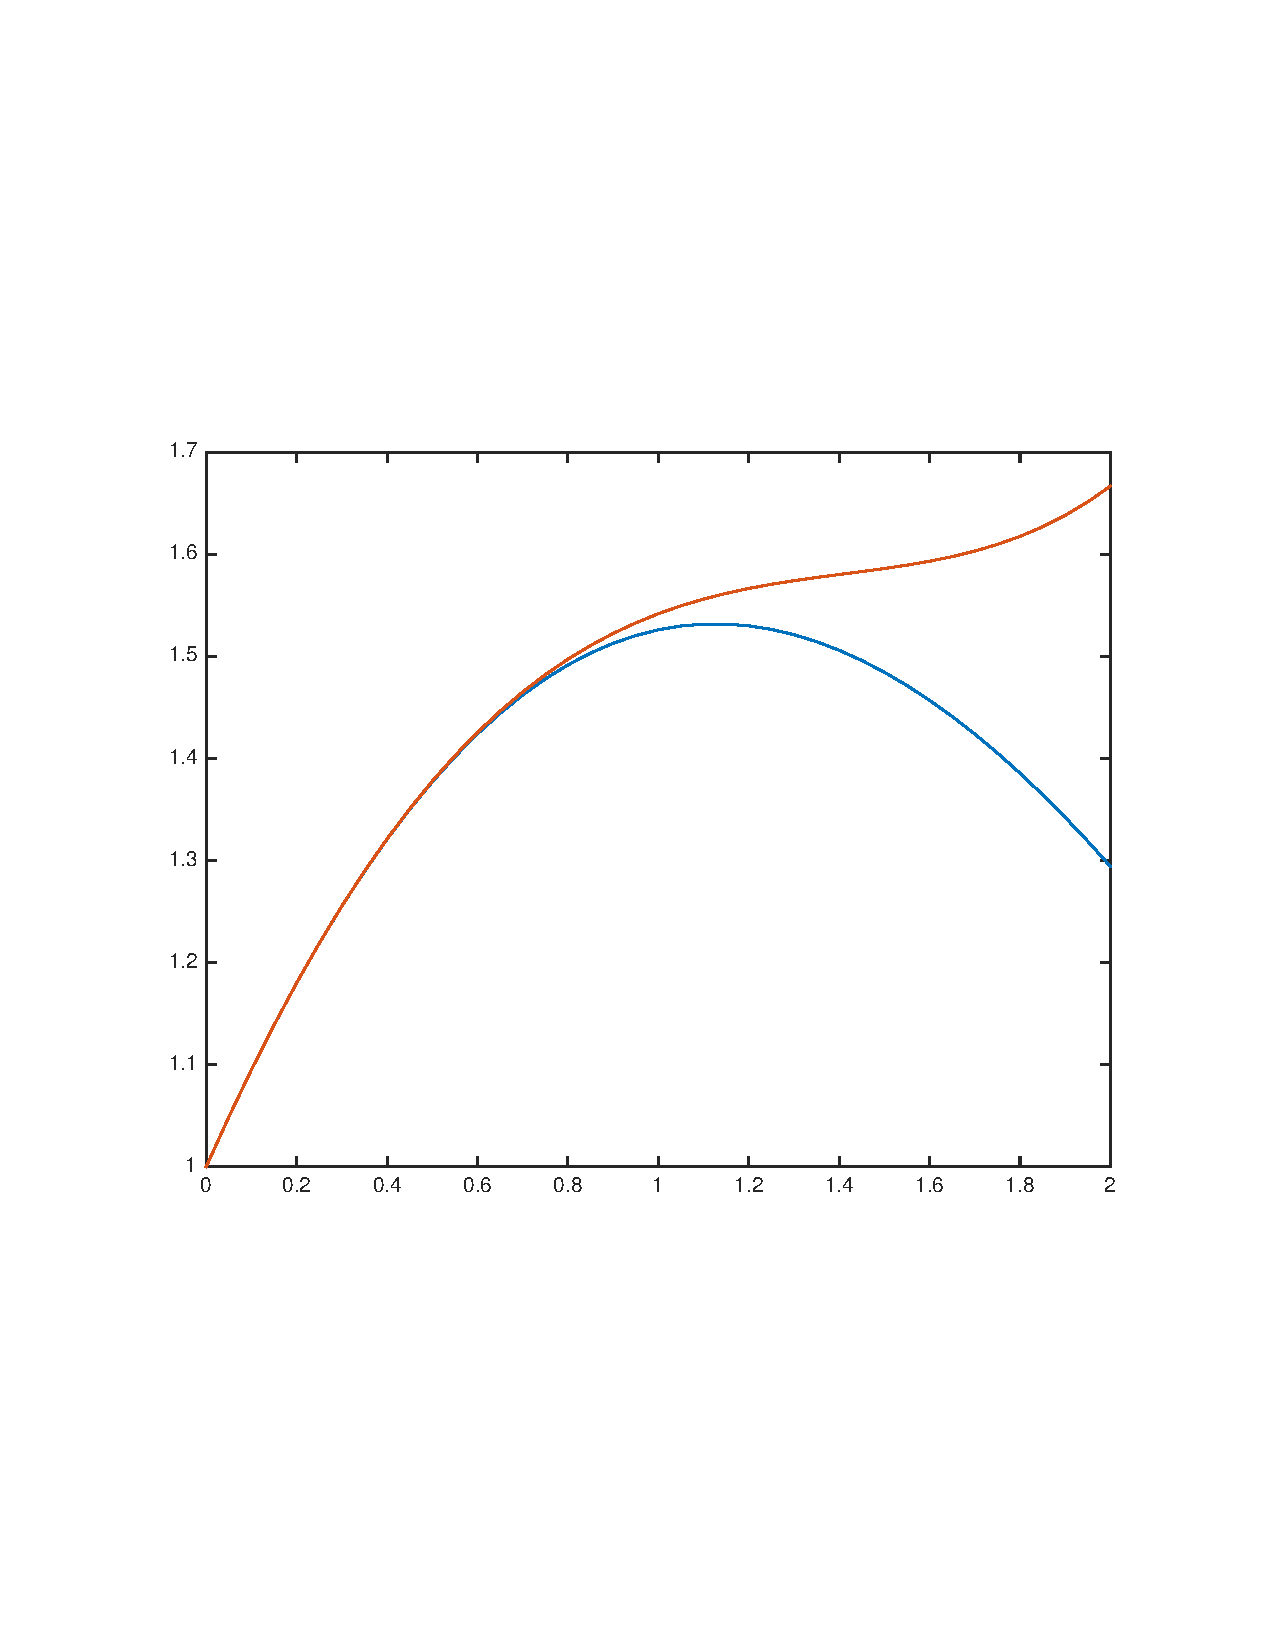
\includegraphics[width = 0.65\textwidth]{power.pdf}
\end{center}
\end{enumerate}
\end{solution}

\end{questions}
\end{document}